\documentclass[tikz,border=3pt]{standalone}
\usepackage[utf8]{inputenc}
\usepackage[T1]{fontenc}
\usepackage{lmodern}
\renewcommand{\familydefault}{\sfdefault}
\usepackage{sansmath}\sansmath
\usepackage{chemfig}
\usepackage{pgfplots}\pgfplotsset{compat=1.18,/pgf/number format/use comma,/pgf/number format/1000 sep={.}}
\usetikzlibrary{arrows.meta,calc,positioning,decorations.pathmorphing,patterns}
% paleta del sitio
\definecolor{nar}{HTML}{E8680C}\definecolor{narc}{HTML}{FFB35C}\definecolor{hielo}{HTML}{FFF3E8}
\definecolor{tinta}{HTML}{1D1D1F}\definecolor{gris}{HTML}{6E6E73}\definecolor{lila}{HTML}{7C5CF0}
\definecolor{azul}{HTML}{2F6FD6}\definecolor{menta}{HTML}{17A673}\definecolor{coral}{HTML}{E8342A}
\begin{document}
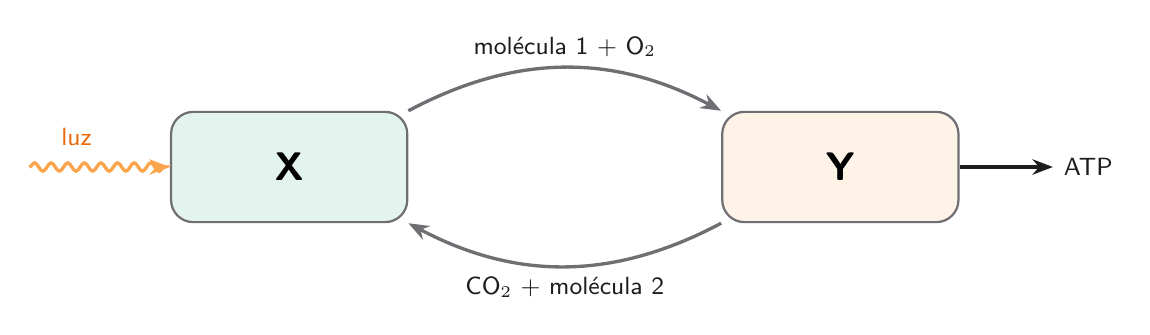
\begin{tikzpicture}[font=\small,>={Stealth[length=2.6mm]}]
\node[draw=gris,fill=menta!12,thick,rounded corners=8pt,minimum width=3.0cm,minimum height=1.4cm,font=\Large\bfseries] (F) at (0,0) {X};
\node[draw=gris,fill=hielo,thick,rounded corners=8pt,minimum width=3.0cm,minimum height=1.4cm,font=\Large\bfseries] (R) at (7,0) {Y};
\draw[->,very thick,gris] (F.north east) to[bend left=28] node[midway,above,text=tinta,align=center] {molécula 1 + O$_2$} (R.north west);
\draw[->,very thick,gris] (R.south west) to[bend left=28] node[midway,below,text=tinta,align=center] {CO$_2$ + molécula 2} (F.south east);
\draw[narc!80!nar,very thick,decorate,decoration={snake,amplitude=1.5pt,segment length=6pt},->] (-3.3,0) -- (F.west);
\node[anchor=south,text=nar] at (-2.7,0.15) {luz};
\draw[->,very thick,tinta] (R.east) -- (9.7,0) node[anchor=west] {ATP};
\end{tikzpicture}
\end{document}
